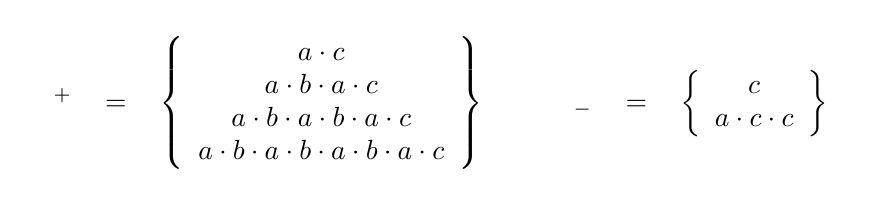
\begin{tikzpicture}

\node[] (logs) at (0,0) {

\begin{tabular}{rcl}
  $\pmlog^+$ & = &
  $\left \{
  \begin{array}{c}
  a \cdot c \\
  a \cdot b \cdot a \cdot c \\
  a \cdot b \cdot a \cdot b \cdot a \cdot c \\
  a \cdot b \cdot a \cdot b \cdot a \cdot b \cdot a \cdot c \\
  \end{array}
  \right \}$
\end{tabular}  
\hspace{5mm}
\begin{tabular}{rcl}
  $\pmlog_-$ & = &
  $\left \{
  \begin{array}{c}
  c \\
  a \cdot c \cdot c
  \end{array}
  \right \}$
\end{tabular}
};

%\node[] (null) at (0,-2) {};

\end{tikzpicture}